% $Id$

One of the most interesting current problems in astrophysics is that of
\emph{dark matter}. Dark matter is so called because it has eluded detection
through its emission or absorption of electromagnetic radiation. Our knowledge
of its existence comes from its gravitational interaction with luminous matter
in the universe. There have been several ideas proposed to explain the nature
of dark matter, chief among these are \emph{weakly interacting massive
particles} (WIMPs) and \emph{massive astrophysical compact halo objects}
(MACHOs)\cite{Griest:1990vu}.  WIMPs, supersymmetric particles produced as a
relic of the big bang, are outside the scope of this thesis\footnote{We refer
to \cite{Griest:1995gs} for a review of the nature of dark matter.}. No
compelling reason exists the think that WIMPs will produce significant
gravitational waves. In this chapter, we review the evidence for dark matter
in the form of MACHOs in the Galactic halo. The nature of MACHOs is unknown;
we review a proposal that suggests that if MACHOs are primordial black holes
(PBHs) formed in the early universe, then some of the PBHMACHOs may be in
binary systems\cite{Nakamura:1997sm}. Searching for gravitational waves from
the inspiral and coalescence of these binary black hole MACHOs (BBHMACHOs) is
the motivation for this thesis.

\section{Dark Matter In The Galactic Halo}
\label{s:darkmatter}

Dark matter is detected by its gravitational interaction with luminous matter.
Strong evidence for the presence of dark matter in the universe comes from the
study of galactic rotation curves: measurements of the velocities of luminous
matter in the disks of spiral galaxies as a function of galactic radius.  
Consider a simple rotational model for the disk of a spiral galaxy.
Consider a star with mass $m_s$ orbiting at radius $r$ in the outer part of
the galaxy's disk. Newtonian dynamics tells us that if the mass inside radius
$r$ is $m_g$ then
\begin{equation}
\frac{Gm_g m_s}{r^2} = \frac{m_s v_s^2}{r}
\label{eq:newtongalaxy}
\end{equation}
where $v_s$ is the velocity of the star and $G$ is the gravitational constant. 
Let us suppose that as we increase $r$, the change in the $m_g$ is negligible,
which is a reasonable assumption towards the edge of the disk of a typical
spiral galaxy.  We can see from equation (\ref{eq:newtongalaxy}) that we would
expect the velocity of stars at the edge of the galactic disk to fall off as 
\begin{equation}
v_s \propto \frac{1}{\sqrt{r}}.
\end{equation}
Galactic rotation curves, determined using the Doppler shift of the $21$~cm
hydrogen line, have been measured for several galaxies\cite{Sancisi:1987}. It
is found that the rotation curves do not fall off as expected. Instead the
rotational velocities of galactic matter are measured to be constant out to
the edge of the visible matter in the disk, as shown in
figure~\ref{f:rotcurves}.  This surprising result suggests that around
80\%--90\% of the matter in spiral galaxies is in the form of dark matter
stretching out at least as far as the visible light.

A typical argument to understand the formation of galactic disks from baryonic
matter considers an initially spherical distribution of baryonic matter
rotating with some angular momentum, $L$. Over time the matter will lose
energy through inelastic collisions. Since the angular momentum of the system
is conserved, the initial distribution must collapse to a rotating disk.  On
the other hand, if the initially spherical distribution is composed of dark
matter insted of baryons, the collisions will be elastic because the dark
matter is weakly interacting. As a result of this, dark matter initially
distributed in an isotropic sphere will maintain this distribution over time.
Since we do not expect a spherical dark matter halo to collapse to a disk, the
simplest possible assumption is that the dark halo is a spherical, isothermal
distribution of dark matter. This suggests that dark matter will be
distributed in an extended halo encompassing the luminous matter of a galaxy.
If we assume that the density of the dark matter
is $\rho(r)$ then the mass within a thin shell of a spherical halo is
\begin{equation}
dM(r) = 4\pi r^2 \rho(r)\, dr,
\label{eq:simplehalodensity}
\end{equation}
where $dr$ is the thickness of the shell.
Using Newtonian dynamics, the velocity $v$ of a particle of mass $m$ at
radius $r$ is
\begin{equation}
\begin{split}
\frac{GM(r)m}{r^2} &= \frac{mv^2}{r} \\
v^2 &= \frac{GM(r)}{r}.
\end{split}
\end{equation}
The galactic rotation curves tell us that the velocity is independent of the
radius, so
\begin{equation}
M(r) = \frac{v^2r}{G}.
\end{equation}
Differentiating this with respect to $r$ and substituting the result into
equation \ref{eq:simplehalodensity}, we obtain
\begin{equation}
\frac{dM(r)}{dr} = \frac{v^2}{G} = 4\pi r^2\rho(r)
\end{equation}
which gives
\begin{equation}
\rho(r) = \frac{v^2}{4\pi r^2 G}.
\label{eq:simplehalodensity2}
\end{equation}
If we assume that the dark and visible matter are in thermal equilibrium, we
may use the measured rotational velocity of local stars about the galactic
center as the velocity of the dark matter. 

We can easily estimate the density of dark matter in the neighborhood of the
Earth $\rho(r_E)$ as follows. The earth is approximately $8$~kpc
from the galactic center and the rotational velocity of objects at this radius
is $v\sim 200$~$\mathrm{km\,s}^{-1}$. Using these values in equation
(\ref{eq:simplehalodensity2}), we find
\begin{equation}
\rho(r_E) = 7.6 \times 10^{-25}\, \mathrm{g}\,\mathrm{cm}^{-3}.
\end{equation}
More sophisticated modeling of the
Galaxy\cite{1995ApJ...449L.123G}, suggests that the local halo density is
\begin{equation}
\rho(r_E) = 9.2_{-3.1}^{+3.8} \times 10^{-25}\, \mathrm{g}\,\mathrm{cm}^{-3}
\end{equation}
or approximately $0.01\,M_\odot\,\mathrm{pc}^{-3}$.

Equation (\ref{eq:simplehalodensity2}) applies only at intermediate radial
distances. The data at small $r$ is consistent with the dark matter having a
constant \emph{core density} $\rho_c$ within a \emph{core radius}
$a$\cite{Rix:1996}. The halo density then becomes
\begin{equation}
\rho(r) = \frac{\rho_c}{1 + \left(\frac{r}{a}\right)^2}.
\label{eq:simplehalodensity3}
\end{equation}
The values of $\rho_c$ and $a$ are obtained by fitting measured galactic
rotation curves to equation (\ref{eq:simplehalodensity3}) using data near the
galactic center.  There is, in fact, no evidence to suggest that halos are
exactly spherical. In fact the halo density may be flattened\cite{Rix:1996}. For a
flattened halo a model of the dark matter density becomes
\begin{equation}
\rho(R,z) = \frac{\rho_c r^2_c}{a^2 + R^2 + z^2/q^2}
\label{eq:simplehalodensity4}
\end{equation}
where $R$ and $z$ are galactocentric cylindrical coordinates and $q$ is a
parameter that describes the flattening of the halo. At present there is no
measurement of the extent of galactic halos beyond the luminous matter. For
the Milky Way it is thought that the halo extends out to a radius of $\sim
50$kpc, athough it is possible that it extens all the way out to the Andromeda
galaxy at $\sim 700$~kpc.

\section{MACHOs in the Galactic Halo}
\label{s:machos}

Galactic rotation curves provide strong evidence that spiral galaxies such
as the Milky Way are surrounded by a large quantity of dark matter, but 
tell us nothing about the nature of this dark matter.  A variety of
candidates have been proposed to explain the nature of dark matter. These
generally fall into two classes. The first class consists of elementary
particles such as axions\cite{Weinberg:1977ma} or weakly interacting massive
particles (WIMPs)\cite{Goodman:1984dc}. 
%Axions are particles proposed to
%explain the lack of CP violation in the strong interaction and WIMPs are
%supersymmetric particles, such as the neutralio.
Such dark matter candidates
are outside the scope of this thesis. Active searches for WIMPs and axions are
underway and we refer to \cite{Griest:1995gs} for a review of the particle
physics dark matter candidates.  The second class of dark matter candidates
are known as \emph{massive astrophysical compact halo objects} or MACHOs.
MACHOs are objects such as brown dwarfs (stars with insufficient mass to burn
hydrogen), red dwarfs (stars with just enough mass to induce nuclear fusion),
white dwarfs (remnants of $1$--$8\,M_\odot$ stars) or black holes located in
the halos of galaxies.  Optical and infrared observations in the early 1990's
were not sensitive enough to constrain the fraction of the halo in
MACHOs\cite{1994MNRAS.266..775K} and the method of \emph{gravitational
lensing} was suggested as a method for detecting halo dark matter in the form
of MACHOs\cite{Paczynski:1985jf}.

\subsection{Gravitational Lensing of Light}
\label{ss:microlensing}

Gravitational lensing is caused by the bending of light around a massive
object. Assume that a MACHO produces a spherically symmetric gravitational
field; the geometry of spacetime around the MACHO satisfies the Schwarzschild
solution. Consider the scattering of light by a MACHO shown in figure
\ref{f:scattering}, where $b$ the \emph{impact parameter} of the light, that
is the minimum distance of the photon to the MACHO.   Recall that the
lightlike orbits of Schwarzschild spacetime satisfy\cite{Wald:1984}
\begin{equation}
\frac{d^2 u}{d\phi^2} + u = \frac{3GM}{c^2}u^2
\label{eq:schphotonorbit}
\end{equation}
where $u = b/r$, $l$ is a constant (of angular momentum), $M$ is the mass
of the MACHO. If $R$ is the size of the
MACHO, then
\begin{equation}
\frac{3GMu^2}{c^2ub} = \frac{3GM}{c^2R} \frac{R}{rb} \ll 1.
\end{equation}
if $b \gg R$. We can solve equation (\ref{eq:schphotonorbit}) perturbatively
in the small parameter $\epsilon = R / b$ as follows. Write
\begin{equation}
u = u_0 + \epsilon u_1 + \cdots
\end{equation}
and substitute into equation (\ref{eq:schphotonorbit}) to get
\begin{equation}
u_0'' + \epsilon u_1'' + \cdots + u_0 + \epsilon u_1 + \cdots = \frac{3GM\epsilon}{c^2R}\left(u_0 + u_1 +
\cdots\right)^2 
\end{equation}
where prime denotes differentiation with respect to $\phi$. At leading order,
\begin{equation}
u_0'' + u_0 = 0
\end{equation}
has solution
\begin{equation}
u_0 = A \sin \left(\phi + \phi_0\right)
\end{equation}
where $A$ and $\phi_0$ are constants. We are free to choose any value for
$\phi_0$ as it simply chooses an orientation for the axes in figure
\ref{f:scattering}, so let $\phi_0 = \pi /2$. Since $\phi = \pi / 2$
gives the distance of closed approach, we find $A = b^{-1}$. Now $u_1$
satisfies
\begin{equation}
\begin{split}
u_1'' + u_1 &= \frac{3GM}{c^2 R} \sin^2 \phi \\
&= \frac{3GM}{2c^2 R}\left(1 - \cos 2\phi\right).
\label{eq:u1eq}
\end{split}
\end{equation}
Inspection suggests a solution of the form
\begin{equation}
u_1 = \frac{3GM}{2c^2 R} + \alpha \cos 2\phi.
\end{equation}
Substituting this into equation (\ref{eq:u1eq}) we find that
\begin{equation}
-4\alpha \cos 2\phi + \frac{3GM}{2c^2 R} + \alpha\cos 2\phi =
\frac{3GM}{2c^2 R} - \frac{3GM}{2c^2 R} \cos 2\phi
\end{equation}
and so $\alpha = GM/2c^2 R$. The solution for $u$, up to first order, is
therefore
\begin{equation}
u = \sin \phi + \frac{GM\epsilon}{2c^2 R}\left(3 + \cos 2\phi\right).
\end{equation}
As $r \rightarrow \infty$, $u \rightarrow 0$ and $\phi \rightarrow - \delta/2$,
so
\begin{equation}
0 = \sin \left(-\frac{\delta}{2}\right) + 
\frac{GM}{2c^2 b} \left(3 + \cos(-\delta)\right)
\end{equation}
For small $\delta$, $\sin(-\delta/2) \approx -\delta/2$ and $\cos(-\delta)
\approx 1$, so
\begin{align}
0 &\approx - \frac{\delta}{2} + \frac{2GM}{c^2 b} \\
\delta &\approx \frac{4GM}{c^2b}
\end{align}
The total deflection of the light is therefore
\begin{equation}
\delta = \frac{4GM}{c^2 b}.
\end{equation}
Suppose a MACHO lens is at a distance $D_\mathrm{SL}$ from a source star and
an observer is at a distance $D_\mathrm{L}$ from the MACHO as shown in figure
\ref{f:macholens}. The then the ray of light from the source that encounters
the MACHO with critical impact parameter $r_\mathrm{E}$ will reach the
observer. Simple geometry, using the small angle approximations, shows that
\begin{equation}
\delta = \theta_\mathrm{S} + \theta_\mathrm{O} =
\frac{r_\mathrm{E}}{D_\mathrm{L}} + \frac{r_\mathrm{E}}{D_\mathrm{SL}} =
\frac{4GM}{c^2r_\mathrm{E}}
\end{equation}
therefore the observer sees the lens light when the ray is at the
\emph{Einstein radius}, $r_\mathrm{E}$, given by
\begin{equation}
r_\mathrm{E} = \sqrt{\frac{4GM}{c^2} \frac{D_\mathrm{SL} D_\mathrm{L}}
{D_\mathrm{SL} + D_\mathrm{L}}}.
\end{equation}
If the source, MACHO and observer are co-linear, as shown in figure
\ref{f:macholens}, then the observer sees a bright ring of radius
$r_\mathrm{E}$ around the MACHO. The angular radius of this ring is the
\emph{Einstein angle},
\begin{equation}
\theta_\mathrm{E} = \sqrt{\frac{4GM}{c^2} \frac{D_\mathrm{SL}}
{D_\mathrm{L}\left(D_\mathrm{SL} + D_\mathrm{L}\right)}}.
\end{equation}
In the realistic case of slight misalignment, then the lensed star will appear
as two small arcs. Consider a MACHO of mass $0.5\,M_\odot$ at a distance of $D
= 25$~kpc lensing a star in the Large Magellanic Cloud (LMC) at a distance of
$50$~kpc. Then
\begin{equation}
\theta_\mathrm{E} = \sqrt{\frac{2GM}{Dc^2}} \approx 10^{-10} \approx 2" \times
10^{-5}
\end{equation}
which too small to be resolved by optical telescopes. Fortunately the lensing
produces an apparent amplification of the source star by a factor
of\cite{1964MNRAS.128..295R}
\begin{equation}
A = \frac{v^2 + 2}{v\sqrt{v^2 + 4}},
\label{eq:lightcurve}
\end{equation}
where $v = \beta / \theta_\mathrm{E}$, and $\beta$ is the angle between the
observer-lens and observer-star lines. Since objects in the halo are in
motion,
\begin{equation}
\beta(t) = \sqrt{ (v_\perp t)^2 + \beta_\mathrm{min}^2 },
\end{equation}
where $v_\perp$ is the transverse velocity of the lens relative to the 
line of sight, $\beta_\mathrm{min}$ is the closest approach of the lens to
the source, and $t$ is the time to the point of closest
approach\cite{Paczynski:1985jf,Griest:1990vu}. 
%Figure \ref{f:lightcurves}
%shows plots of the amplification factor $A(t)$, known as a \emph{light curve},
%obtained for several values of $\beta_\mathrm{min} / \theta_\mathrm{E}$.
Searches for the amplification of stars caused by gravitational lensing of
$\theta_\mathrm{E} \sim $ micro arc seconds are referred to as
\emph{gravitational microlensing surveys.} Such surveys measure
magnification of the star and the duration of the microlensing event. 
Unfortunatley it is not possible to determine the \emph{size} of the
the lens from these measurements.

\subsection{Gravitational Microlensing Surveys}

Several research groups are engaged in the search for microlensing events from
dark matter\cite{Alcock:2000ph,Afonso:2002xq}. By monitoring a large
population of well resolved background stars such as the LMC, constraints can
be placed on the MACHO content of the halo. The MACHO project has conducted a
5.7 year survey monitoring 11.9 million stars in the LMC to search for
microlensing events\cite{Alcock:2000ph} using an automated search algorithm to
monitor the light curves of LMC stars. Optimal filtering is used to search for
light curves with the characteristic shape given by equation
(\ref{eq:lightcurve}).

Since the effect of microlensing is achromatic, light curves are monitored in
two different frequency bands to reduce the potential background sources
which may falsely contribute to the microlensing rate. Background events
include variable stars in the LMC (known as bumpers\cite{1996astro.ph..6165A}), 
which can usually be rejected as the fit of the light curves to true
microlensing curves is poor. Supernovae occuring behind the LMC are the most
difficult to cut from the analysis. The MACHO project reported 28 candidate
microlensing events in the 5.7 year survey of which 10 were thought to be
supernovae behind the LMC and 2--4 were expected from lensing by known stellar
populations.  They report an excess of 13--17 microlensing events, depending
on the selection criteria used.

The \emph{optical depth}, $\tau$, is the probability that a given source star
is amplified by a $A > 1.34$\cite{Paczynski:1985jf}. This is just the
probability that the source lies on the sky within a disk of radius
$\theta_\mathrm{E}$ around a microlensing object and is given
by\cite{Alcock:1995zx}
\begin{equation}
\tau = \frac{4\pi G}{c^2} \int_0^{L} \rho(l) \frac{l(L - l)}{L}\,dl,
\end{equation}
where $L = D_\mathrm{SL} + D_\mathrm{L}$ is the observer-star distance and $l
= D_\mathrm{L}$ is the observer-lens distance. For the spherical halo given in
equation (\ref{eq:simplehalodensity3}) with density
\begin{equation}
\rho(r) = 0.0079 \frac{R_0^2 + a^2}{r^2 + a^2} \,M_\odot\, pc^{-3},
\end{equation}
where $R_0 = 8.5$~kpc is the Galactocentric radius of the Sun and a galactic
core radius of $a = 5$~kpc, the predicted optical depth towards the LMC
(assumed to be at $50$~kpc) is\cite{Alcock:1995zx}
\begin{equation}
\tau_\mathrm{LMC} = 4.7 \times 10^{-7}.
\end{equation}
The optical depth towards the LMC measured by the MACHO project microlensing
surveys is
\begin{equation}
\tau_\mathrm{LMC} = 1.2_{-0.3}^{+0.4} \times 10^{-7}.
\end{equation}
This suggests that the fraction of the halo in MACHOs is less that $100\%$,
but does not exclude a MACHO halo.

The number of observed MACHO events and the time scales of the light curves
can be compared with various halo models. The MACHO project has performed a
maximum-likelihood analysis in which the halo MACHO fraction $f$ and MACHO
mass $m$ are free parameters. For the standard spherical halo, they find the
most likely values are $f = 20\%$ and $m = 0.45\,M_\odot$. The $95\%$
confidence interval of on the MACHO halo faction is $f = 8\%$--$50\%$ and the
$95\%$ confidence interval of on the MACHO mass is $0.15$--$0.9\,M_\odot$. The
total mass in MACHOs out to $50$~kpc is found to be $9_{-3}^{+4} \times
10^{10}\,M_\odot$, independent of the halo model\cite{Alcock:2000ph}.  The
EROS collaboration has recently publish results of a search for microlensing
events towards the Small Magellanic Cloud (SMC)\cite{Afonso:2002xq}. These
results further constrain the fraction a standard halo composed of MACHOs of
mass $2 \times 10^{-7}$--$1\, M_\odot$ to less than $25\%$, but do not rule
out a MACHO component of the halo.

\section{Gravitational Waves from Binary Black Hole MACHOs}
\label{s:bbhmacho}

Since the microlensing surveys have shown that $\sim 20\%$ of the halo dark
matter may be in the form of $\sim 0.5\,M_\odot$ MACHOs, it is natural to ask
what the MACHOs may be. As we mentioned above, it has been proposed that
MACHOs could be baryonic matter in the form of brown dwarfs, objects lighter
than $\sim 0.1\,M_\odot$ that do not have sufficient mass to sustain fusion,
however, this is inconsistent with the observed masses of MACHOs. The fraction
of the halo in red dwarfs, the faintest hydrogen burning stars with masses
greater than $\sim 0.1\,M_\odot$, can be constrained using the Hubble Space
Telescope. Hubble observations may also be used to constrain the fraction of
the halo in brown dwarfs. The results indicate that brown dwarfs make up less
than $\sim 3\%$ and red dwarfs less than $\sim 1\%$ of the
halo\cite{Graff:1995ru,Graff:1996rz}.  A third possible candidate for baryonic
MACHOs is a population of ancient white dwarfs in the halo. White dwarfs are
the remnants of stars of mass $1$--$8\,M_\odot$ and have masses of $\sim
0.6\,M_\odot$. Although they seem to be natural candidates for MACHOs,
searches for halo white dwarfs have been conducted and no candidates have
found\cite{2002A&A...389L..69G,2002ApJ...573..644N,Creze:2004gs}.
Creeze~\emph{et~al.} combined the results of previous surveys to find that
$4\%$ ($95\%$ confidence level) of the halo is in the form of white
dwarfs\cite{Creze:2004gs}. 

It is possible that there is an over dense clump of MACHOs in the direction of
the LMC\cite{1996ApJ...473L..99N}, the lenses are located in the LMC
itself\cite{Salati:1999gd} or in the disk of the galaxy\cite{Evans:1997hq}. 
If the MACHOs detected by microlensing are truly in the halo, however, it is
possible that MACHOs are non-baryonic matter such as black holes
\cite{Finn:1996dd,Nakamura:1997sm}. Black holes of mass $\sim 0.5\,M_\odot$
could not have formed as a product of stellar evolution and so they must have
been formed in the early universe\cite{1967SvA....10..602Z,1974MNRAS.168..399C}.
Several mechanisms have been proposed to form primordial black holes with the
masses consistent with the MACHO observations. These include multiple scalar
fields during inflation\cite{Yokoyama:1995ex}, chaotic 
inflation\cite{Yokoyama:1999xi} or reduction of the speed of sound during the
QCD phase transition\cite{Jedamzik:1996mr}. We do not consider these formation
mechanisms in detail here, it is sufficient for our purposes PBHs with masses
consistent with microlensing observations can form.  If the MACHOs are
primordial black holes then there must be a large number of them in the halo. 
The total mass in MACHOs out to $50$~kpc is $9\times 10^{10}\,M_\odot$, as
measured by microlensing surveys. If these are $0.5\,M_\odot$ PBHs then there
will be at least $\sim 1.8 \times 10^{11}$ PBHs in the halo. With such a large
number of PBHs in the halo it is natural to assume that some of these may be
in binary systems.

Nakamura~\emph{et~al.} considered PBHs formed when the scale factor of the
universe $R$, normalized to unity at the time of matter-radiation equality,
is\cite{Nakamura:1997sm}
\begin{equation}
R_f = \sqrt{GM_\mathrm{BH}}{c^2L_\mathrm{eq}} =
1.2\times 10^{-8} \left(\frac{M_\mathrm{BH}}{M_\odot}\right)^\frac{1}{2}
(\Omega h^2),
\end{equation}
where $L_\mathrm{eq}$ is the Hubble horizon scale at the time of
matter-radiation equality, $\Omega$ is the fraction of the closure density in
PBHs and $h$ is the Hubble parameter in units of $100$~km~s$^{-1}$. The age
and temperature of the universe at this epoch are $\sim 10^{-5}$~seconds and
$\sim 1$~GeV, respectively. By considering a pair of black holes that have
decoupled from the expansion of the universe to form a bound system
interacting with a third black hole, which gives the pair angular momentum to
form a binary, they showed that the distribution of the semi-major axis, $a$,
and eccentricity, $e$ of a population of binary black hole MACHOs is
\begin{equation}
f(a,e)\, da\, de = 
\frac{ 3ea^{\frac{1}{2}} }
{ 2\bar{x}^{\frac{3}{2}} (1-e^2)^{\frac{3}{2}}  } \, da\, de 
\label{eq:semieccdist}
\end{equation}
where $\bar{x}$ is the mean separation of the black hole MACHOs at the time of
matter-radiation equality, given by
\begin{equation}
\bar{x} = 1.1 \times 10^{16} \left(\frac{M}{M_\odot}\right)^{\frac{1}{3}}
\left(\Omega h^2\right)^{-\frac{4}{3}} \,\mathrm{cm},
\end{equation}
The coalescence time of a binary by the emission of gravitational waves is
approximately given by
\cite{Peters:1964}
\begin{equation}
t = t_0 \left(\frac{a}{a_0}\right)^4 \left(1 - e^2\right)^{\frac{7}{2}},
\label{eq:peters}
\end{equation}
where $t = 10^{10}$~years and
\begin{equation}
a_0 = 2 \times 10^{11}
\left(\frac{M}{M_\odot}\right)^{\frac{3}{4}}\,\mathrm{cm}
\end{equation}
is the semimajor axis of a binary with circular orbit which coalesces in time
$t_0$. Integrating equation (\ref{eq:semieccdist}) for fixed $t$ using equation
(\ref{eq:peters}), Nakamura~\emph{et~al.} found the probability distribution
for the coalescence the time $f_t(t)$ is
\begin{equation}
f_t(t)\,dt = \frac{3}{29}\left[
\left(\frac{t}{t_\mathrm{max}}\right)^{\frac{3}{37}} -
\left(\frac{t}{t_\mathrm{max}}\right)^{\frac{3}{8}}\right] \frac{dt}{t},
\end{equation}
where $t_\mathrm{max} = t_0(\bar{x}/a_0)^4$. The number of coalescing binaries
with $t \sim t_0$ is then $\sim 5 \times 10^{8}$ for $\Omega h^2 = 0.1$, so
the event rate of coalescing binaries is $\sim 5 \times 10^{-2}$ events per
year per galaxy. Ioka~\emph{et~al.} performed more detailed studies of binary
black hole MACHO formation in the early universe\cite{Ioka:1998nz} and found
that, within a $50\%$ error, the distribution function and the rate of
coalescence given in \cite{Nakamura:1997sm} agree with numerical simulations.
The event rate of coalescing binary black hole MACHOs is therefore
\begin{equation}
R_\mathrm{BBHMACHO} = 5\times 10^{-2}\times 2^{\pm
1}\,\mathrm{yr}^{-1}\,\mathrm{galaxy}^{-1}.
\end{equation}
This rate is significantly higher than the coalescence rate of
binary neutron stars, which is\cite{Kalogera:2004tn}
\begin{equation}
R_\mathrm{BNS} = 8.3\times 10^{-5}\times 2^{\pm
1}\,\mathrm{yr}^{-1}\,\mathrm{galaxy}^{-1}.
\end{equation}
It must be emphasised that several neutron star binaries have been
observed, but there are no observations of black hole MACHO binaries.

The distance to which we can detect a binary inspiral is usually expressed in
terms of the \emph{characteristic strain}, $h_\mathrm{char}$ of the binary. This
represents the intrinsic amplitude of the signal at some frequency times the
square-root of the number of cycles over which the signal is observed at that
frequency
\begin{equation}
h_\mathrm{char}(f) = |f \tilde{h}(f)| \approx h \sqrt{n}
\end{equation}
 For an inspiral signal this is given by\cite{Thorne:1982cv}
\begin{equation}
h_\mathrm{char}(f)  =  4 \times 10^{-21} \left(\mathcal{M}{M_\odot}\right)^\frac{5}{56}
\left(\frac{f}{100\,\mathrm{Hz}}\right)^{-\frac{1}{6}} \left(\frac{r}{20\,
\mathrm{Mpc}}\right)^{-1},
\end{equation}
where $r$ is the distance to the binary and $\mathcal{M}$ is the chirp mass.
For comparison with signal strength, the detector sensitivity is better
expressed in terms of the root mean square (RMS) dimensionless strain per
logarithmic frequency interval
\begin{equation}
h_\mathrm{rms} = \sqrt{f |\tilde{s}(f)|^2} = \sqrt{f S_n(f)},
\end{equation}
where $s$ is the detector strain output in the absence of a gravitational wave
signal and $S_n(f)$ is the power spectral density of $s$. If the value of $h_c
> h_\mathrm{rms}$, then the binary will be
detectable. Figure~\ref{f:machosensitivity} shows the characteristic strain of
a binary consisting of two $0.5\,M_\odot$ black holes at $10$~Mpc compared to
the RMS noise for initial LIGO. It can be seen that the inspiral signal lies
significantly above the noise, so these MACHO binaries could be excellent
source for initial LIGO. Nakamura~\emph{et~al.} showed that the rate of MACHO
binaries could be as high as $3$~yr$^{-1}$ at a distance of
$15$~Mpc\cite{Nakamura:1997sm}, under their model assuptions.

\section{Binary Black Hole MACHO Population Model}
\label{s:bbhmachopopulation}

The goal of this thesis is to search for gravitational waves from binary black
hole MACHOs described in the previous section. In the absence of a detection,
however, we wish to place an \emph{upper limit} on the rate of binary black
hole MACHO inspirals in the galaxy. We can then compare the predicted rate
with that determined by experiment. We will see later that in order to
determine an upper limit on the rate, we need to measure the \emph{efficiency}
$\varepsilon$ of our search to binary black hole MACHOs in the galactic halo.
We do this using a Monte Carlo simulation which generates a population of
binary black hole MACHOs according to a given probability density function
(PDF) of the binary black hole MACHO parameters. Using the set of parameters
generated by sampling the PDF, we can simulate the corresponding inspiral
waveforms on a computer. We then digitally add the simulated waveforms to the
output of the gravitational wave detector. By analyzing the interferometer
data containing the simulated signals, we can determine how many events from
the known source distribution we find. The efficiency of the
search is then simply
\begin{equation}
\varepsilon = 
\frac{\textrm{number of signals found}}{\textrm{number of signals injected}}.
\end{equation}
Recall that an inspiral waveform is described by the following nine 
parameters:
\begin{equation*}
\begin{split}
t_c &\quad \textrm{the end time of the inspiral}, \\
m_1 &\quad \textrm{the mass of the first binary component}, \\
m_2 &\quad \textrm{the mass of the second binary component}, \\
\iota &\quad \textrm{the inclination angle of the binary}, \\
\phi_0 &\quad \textrm{the oribital phase of the binary}, \\
\psi &\quad \textrm{the polarization angle of the binary}, \\
(\theta,\varphi) &\quad \textrm{the coordinates of the binary},\\
r  &\quad \textrm{the distance to the binary}.
\end{split}
\end{equation*}
To simulate a population of BBHMACHOs in the halo we need to generate a list
of these parameters that correctly samples their distributions.

We first address the generation of inspiral end time, $t_c$. The nature of the
noise in the interferometers changes with time, as does the orientation of the
detectors with respect to the galaxy as the earth rotates about its axis over
a sidereal day. To sample the changing nature of the detector output, the
Monte Carlo population that we generate contains many inspiral signals with
end times distributed over the course of the science run. We generate values
of $t_c$ at fixed intervals starting from a specified time $t_0$. The fixed
interval is chosen to be $2048+\pi \approx 2051.141592653$~sec. This
allows us to inject a significant number of signals over the course of the two
month run with the signals far enough apart that they do not dominate the
detector output. The interval is chosen to be non-integer to avoid any
possible periodic behavior associated with data segmentation.
The start time for the Monte Carlo, $t_0$, is chosen from a uniform random
distribution in the range $t_\mathrm{start} - 2630/\pi \le t_0 \le
t_\mathrm{start}$, where $t_\mathrm{start}$ is the time at which the science
run begins. We stop generating inspiral parameters when $t_c > t_\mathrm{end}$
the time at which the second science run ends. For each generated end time,
$t_c$ we generate the other inspiral waveform parameters.

We obtain the distribution of the mass parameters $(m_1,m_2)$ from the
microlensing observations of MACHOs in the galactic halo, described in section
\ref{ss:microlensing}, which suggest that the most likely MACHO mass is between
$0.15$ and $0.9\,M_\odot$. In the absence of further information on the mass
distribution we simply draw each component mass from a uniform
distribution in this range. We increase the range slightly to better measure
the performance of our search at the edge of the parameter space. We also note
that the search for binary neutron stars covers the mass range $1$ to
$3\,M_\odot$, so we continue the BBHMACHO search up to $1\,M_\odot$ rather
than terminating it at $0.9\,M_\odot$. We therefore generate each BBHMACHO
mass parameter, $m_1$ or $m_2$, from a uniform distribution of masses between
$0.1$ and $1.0\,M_\odot$.

The angles $\iota$ and $\phi_0$ are generated randomly to reflect a uniform
distribution in solid angle; $\cos \iota$ is uniform between $-1$ and $1$ and
$\phi_0$ is uniform between $0$ and $2\pi$. The polarization angle $\psi$ is
also generated from a uniform distribution between $0$ and $2\pi$.

To generate the spatial distribution of BBHMACHOs, we assume that the
distribution in galactocentric cylindrical coordinates, $(R,\theta,z)$,
follows the halo density given by equation (\ref{eq:simplehalodensity4}),
that is,
\begin{equation}
\rho(r) \propto \frac{1}{a^2 + R^2 + z^2/q^2}
\end{equation}
where $a$ is the halo core radius and $q$ is the halo flattening parameter. We
can see that this distribution is independent of the angle $\theta$, so we
generate $\theta$ from a uniform distribution between $0$ and $2\pi$.  If
we make the coordinate change $z/q \rightarrow z$, then we may obtain a
probability density function (PDF) for the spatial distribution of
the MACHOs given by
\begin{equation}
f(R,z)\,R\, dR\, dz \propto \frac{1}{a^2 + R^2 + z^2}\,R\, dR\, dz.
\label{eq:spacepdf}
\end{equation}
We wish to randomly sample this PDF to obtain the spatial distribution of
the BBHMACHOs. Once we have obtained a value of the new coordinate $z$, we
simply scale by $q$ to obtain the original value of $z$. Recall that for a
probability density function $f(x)$ the cumulative distribution $F(X)$
given by
\begin{equation}
F(X) = \int_{-\infty}^X f(x)\, dx
\end{equation}
is uniformly distributed over the interval $[0,1]$ for all $f(x)$. Hence a
random variable $u$ uniformly distributed between $0$ and $1$ can be
interpreted as a random sample of $F(X)$. If we generate a value of $u$,
uniform between $[0,1]$, we can solve 
\begin{equation}
\int_{-\infty}^x f(x')\, dx' = u
\label{eq:goldenrule}
\end{equation}
to obtain the value of $x$. Notice, however, that PDF in equation
(\ref{eq:spacepdf}) is a function of the two random variables $R$ and $z$,
rather than a single variable $x$ as in equation (\ref{eq:goldenrule}).
Let us make the coordinate change
\begin{equation}
\begin{split}
R &= r \cos \varphi, \\
z &= r \sin \varphi \\
\label{eq:probcoordtrans}
\end{split}
\end{equation}
and so
\begin{equation}
\begin{split}
\tan \varphi &= \frac{z}{R}, \\
r^2 &= R^2 + z^2. \\
\end{split}
\end{equation}
Equation (\ref{eq:spacepdf}) becomes
\begin{equation}
\begin{split}
\mathcal{K} \int\int \frac{1}{a^2 + R^2 + z^2}\,R\, dR\, dz 
&= \mathcal{K} \int\int \frac{r\cos\varphi}{a^2+r^2}\,r\, dr \, d\varphi \\
&= \mathcal{K} \int_{-1}^{1} d\sin\varphi \int_0^{r_{\mathrm{max}}} \frac{r^2}{a^2+r^2}\, dr \\
&= \mathcal{K} \left[\sin\varphi\right]_{-1}^1 \left[r -
a\arctan\left(\frac{r}{a}\right)\right]_0^{r_{\mathrm{max}}},
\end{split}
\label{eq:bothpdfs}
\end{equation}
where $r_\mathrm{max} = 50$~kpc is the extent of the halo and $\mathcal{K}$ is
a constant that normalizes the PDF to unity. We can see immediately from
equation (\ref{eq:bothpdfs}) that $\sin\varphi$ is uniformly
distributed between $-1$ and $1$. Now consider the PDF for $r$ given by
\begin{equation}
f(r) = \mathcal{K} \left[r - a\arctan\left(\frac{r}{a}\right)\right]_0^{r_{\mathrm{max}}}
\end{equation}
with normailzation constant
\begin{equation}
\mathcal{K} = 
\left[R_\mathrm{max} -
a\arctan\left(\frac{R_\mathrm{max}}{a}\right)\right]^{-1}
\end{equation}
To sample the distribution for $r$, generate a random variable $u$
uniform between $0$ and $1$ and find the root of
\begin{equation}
r - a\arctan\left(\frac{r}{a}\right) - u \left[R_\mathrm{max} -
a\arctan\left(\frac{R_\mathrm{max}}{a}\right)\right] = 0.
\label{eq:rroot}
\end{equation}
We can see that the value of $r$ that solves equation (\ref{eq:rroot}) must
lie between $0$ and $R_\mathrm{max}$ and that the left hand side is a
monotonically increasing function of $r$. We may therefore use a simple 
bisection to solve for the value of $r$. The values of $r$
and $\varphi$ are easily inverted for $R$ and $z$ using equation
(\ref{eq:probcoordtrans}). 

This method was implemented in lalapps\_minj and figure~\ref{f:m1_hist} shows
a histogram of the first mass parameter generated the by the Monte Carlo code.
It can be seen that this is uniform between $0.2$ and $1.0\,M_\odot$, as
expected. Figures \ref{f:spherical_cartesian} shows the spatial distribution
of BBHMACHO binaries for a spherical, $q=1$, halo that extends to
$R_\mathrm{max} = 50\,\mathrm{kpc}$ with a core radius of $a = 5$~kpc.  Since
the software that simulates inspiral waveforms expects the position of the
inspiral to be specified in equatorial coordinates, the population Monte Carlo
code also generates the coordinates of the inspiral as longitude, latitude and
distance from the center of the earth, as shown in figure
\ref{f:spherical_equatorial}.  We will return to the use of population Monte
Carlos in chapter \ref{ch:result}.

\newpage

\begin{figure}[p]
\label{f:rotcurves}
\begin{center}
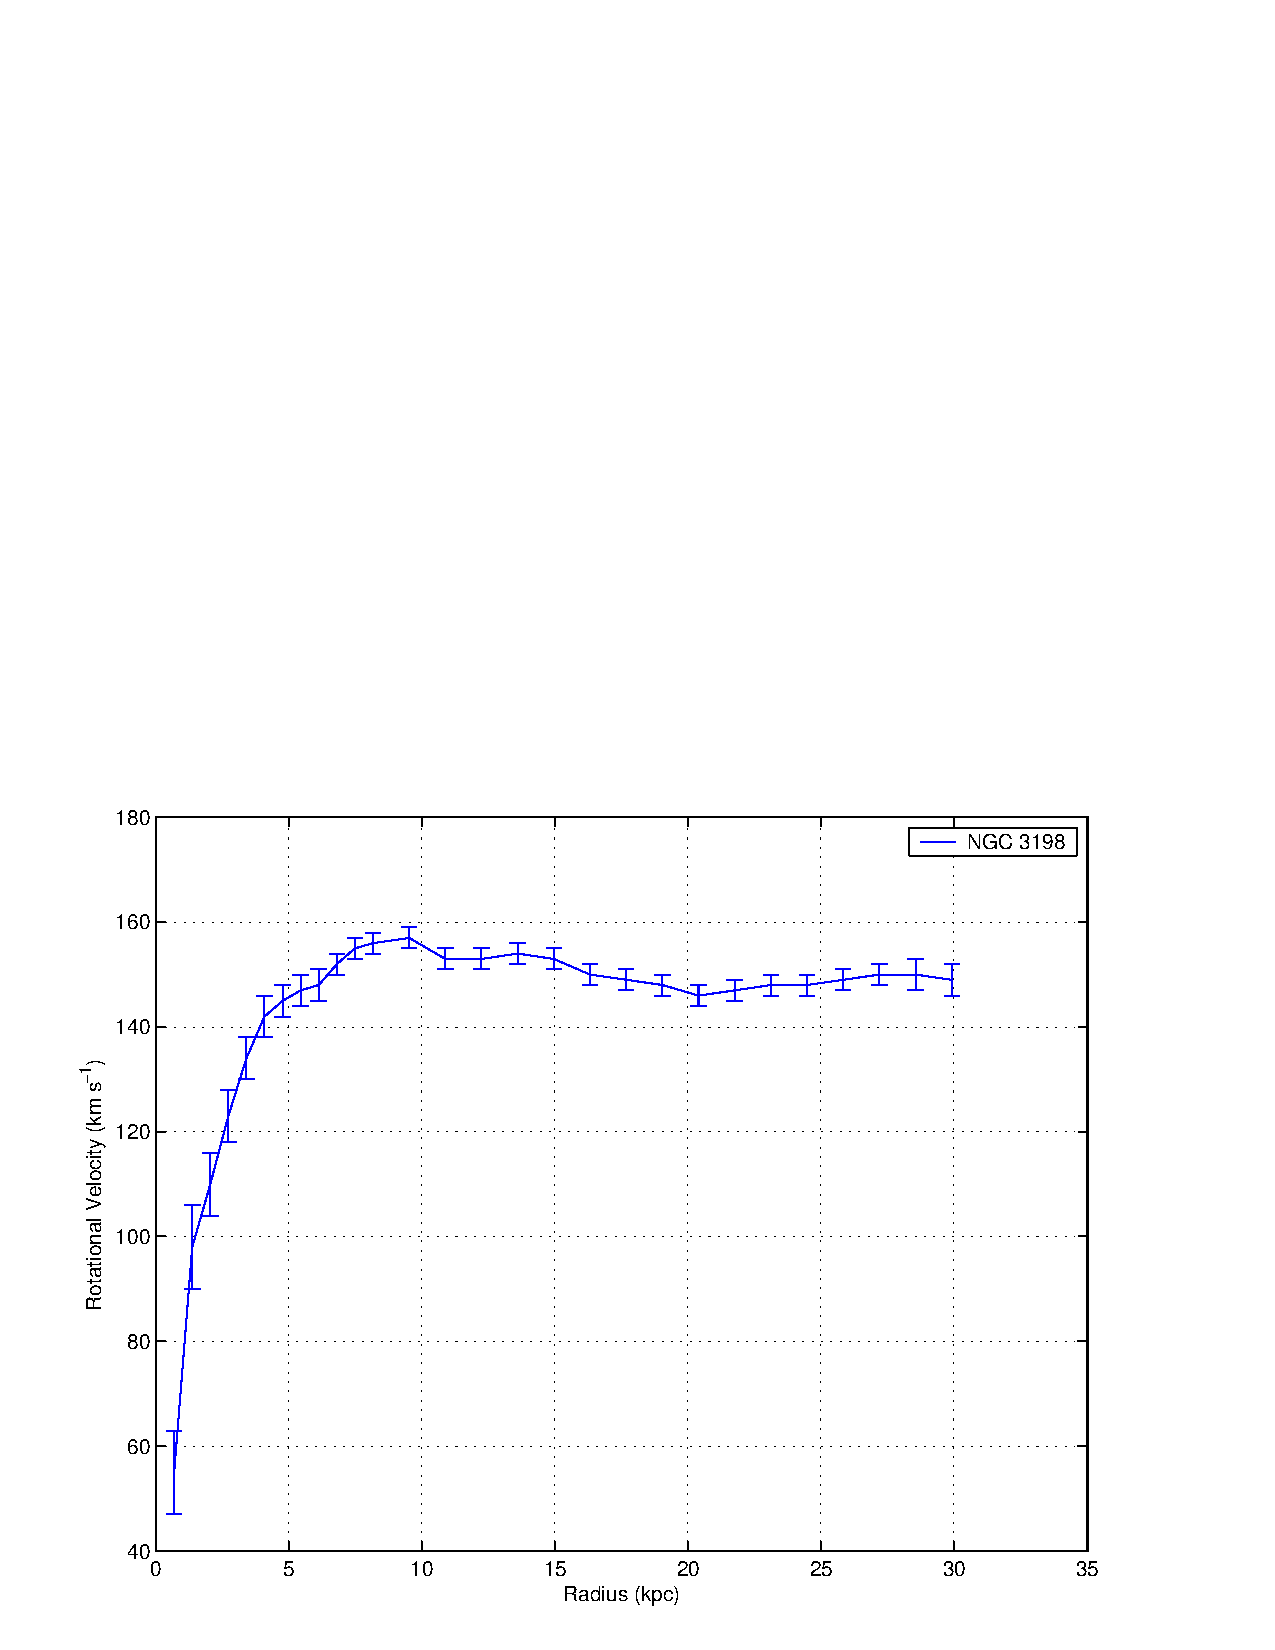
\includegraphics[width=\linewidth]{figures/macho/ngc3198}
\end{center}
\caption[H1 Rotation Curve of NGC 3198]{%
The results of observations of the hydrogen $21$~cm line of the spiral galaxy
NGC 3198 show that the rotation curve is flat out to the last measured point
at $30$~kpc\cite{1989A&A...223...47B}. This implies a large discrepancy
between the observed rotation curve and that predicted from light
observations.
}
\end{figure}

\begin{figure}[p]
\label{f:scattering}
\begin{center}
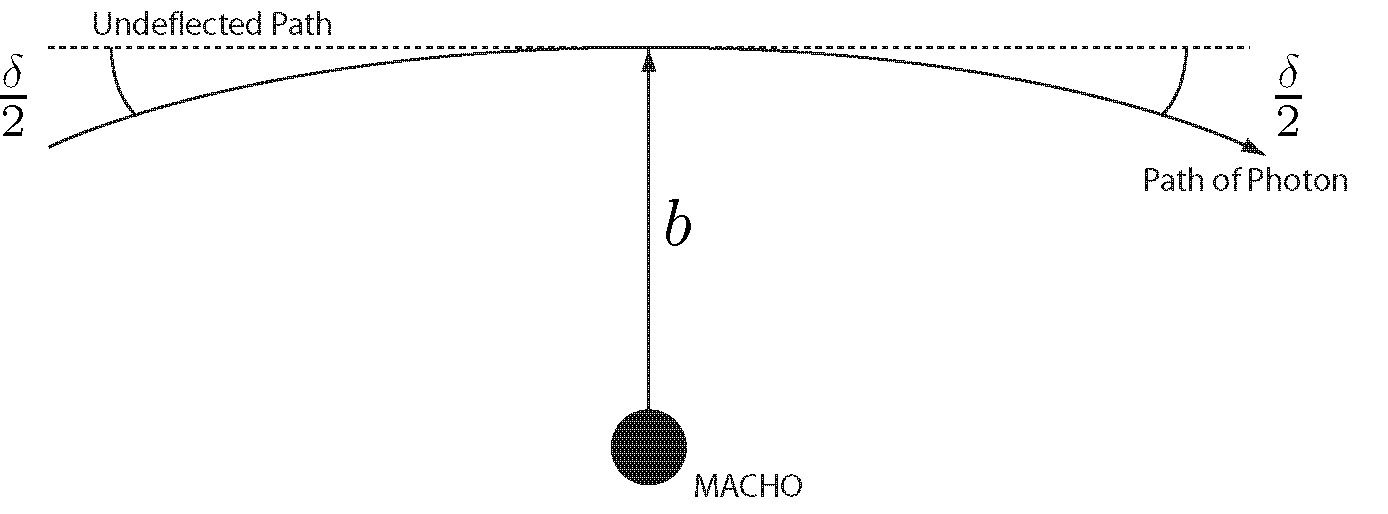
\includegraphics[width=\linewidth]{figures/macho/scattering}
\end{center}
\caption[Scattering of Light in Schwarzschild Spacetime]{%
A photon will be scattered by the curvature of spacetime caused to the
gravitational field of a MACHO. If the closest approach of the photon is 
$b$, it will be deflected by an angle $\delta = 4GM / c^2 b$.
}
\end{figure}

\begin{figure}[p]
\label{f:macholens}
\begin{center}
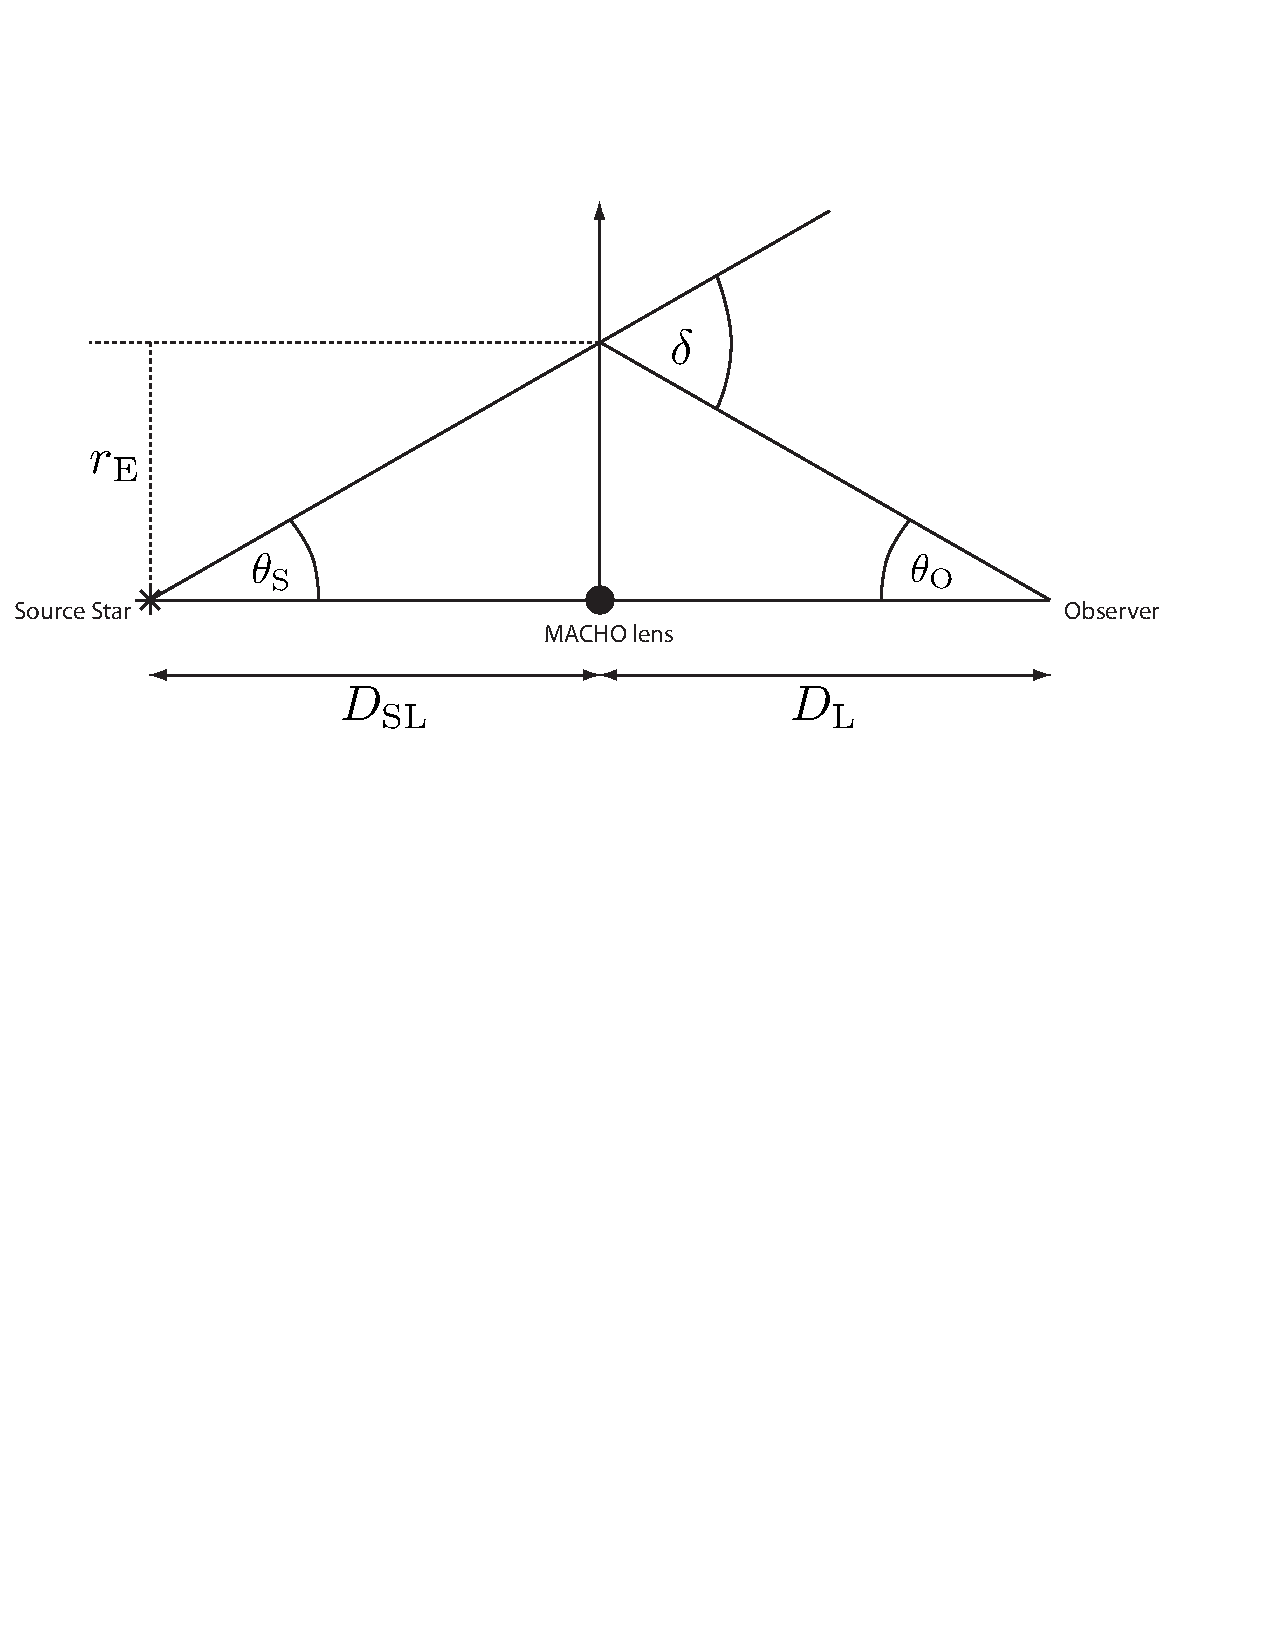
\includegraphics[width=\linewidth]{figures/macho/lensing}
\end{center}
\caption[Gravitational Lensing of Light By a MACHO]{%
The geometry of microlensing of light from a source star by a MACHO showing
the definition of the Einstein radius, $r_\mathrm{E}$.
}
\end{figure}

\begin{figure}[p]
\label{f:machosensitivity}
\begin{center}
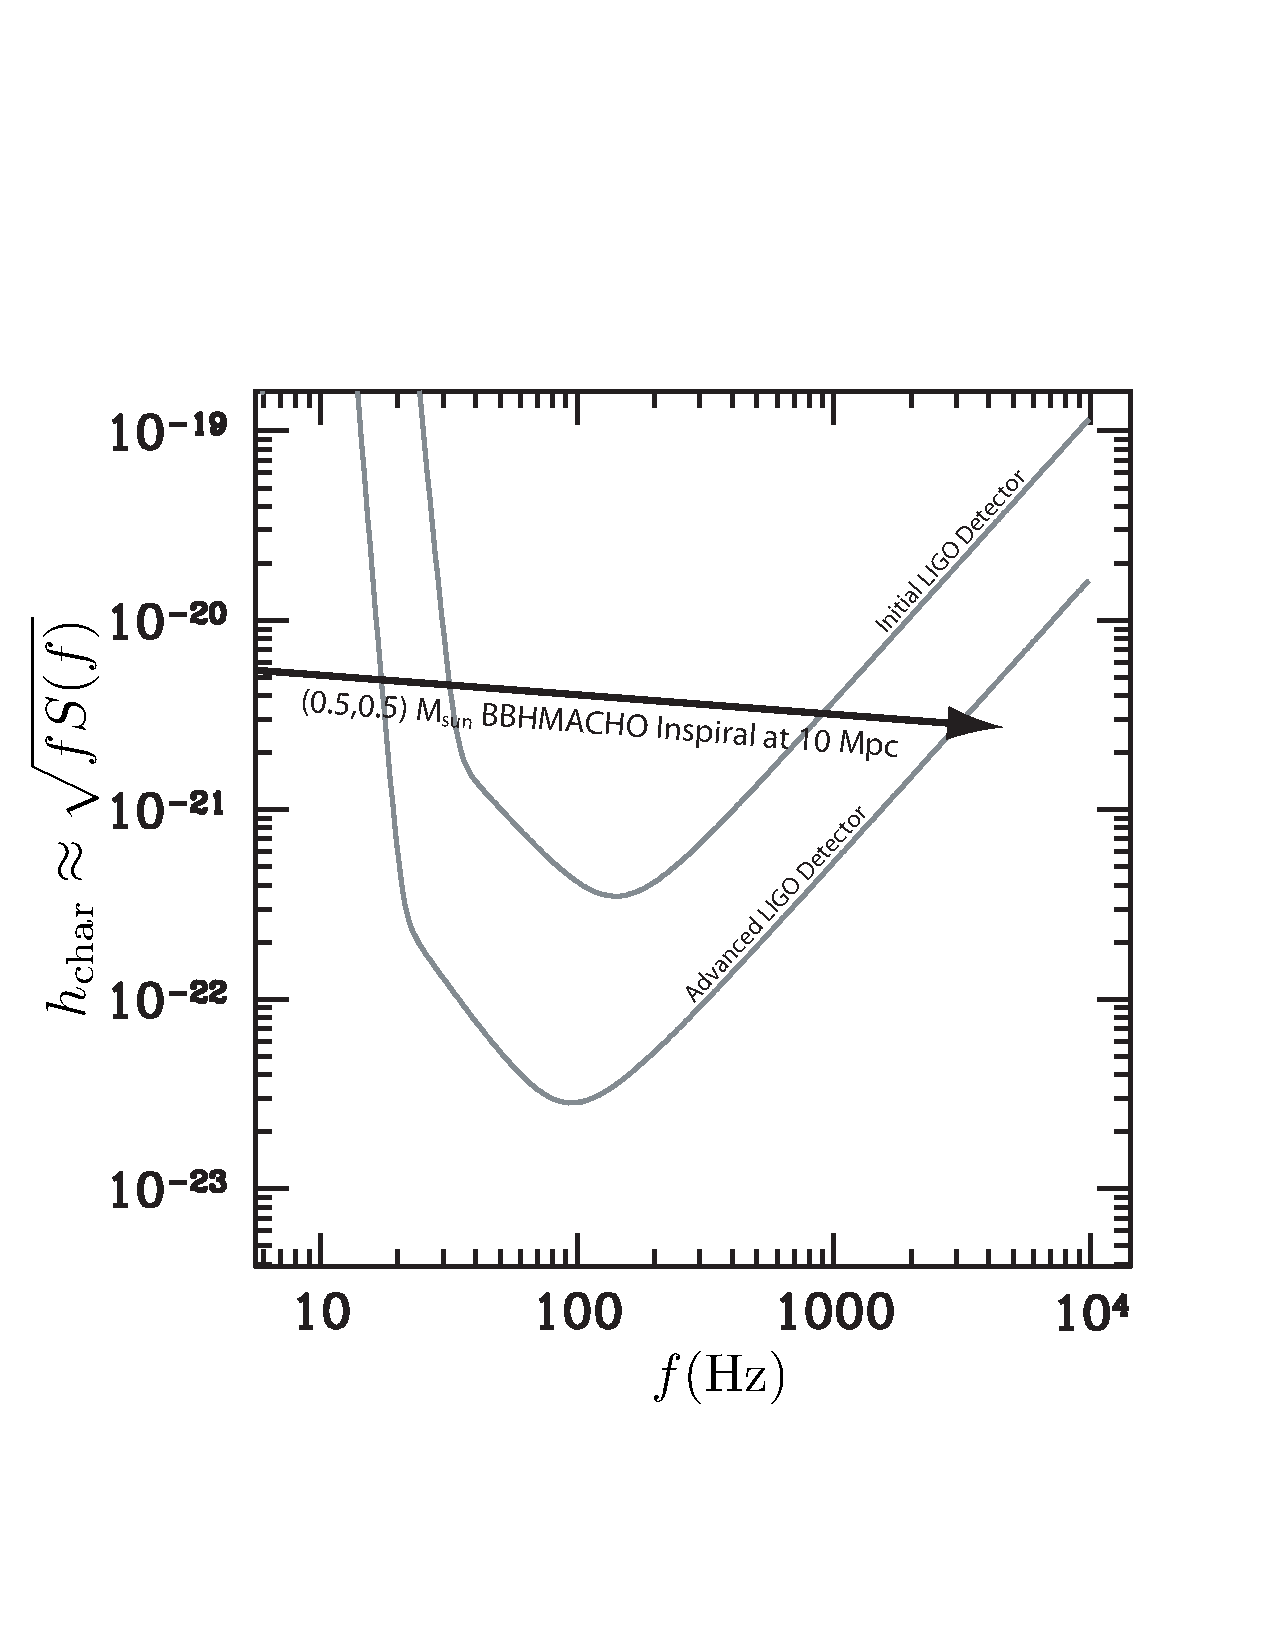
\includegraphics[width=\linewidth]{figures/macho/noisecurves}
\end{center}
\caption[Sensitivity of LIGO to a Binary Black Hole MACHO Inspiral]{%
The sensitivity of LIGO to a binary black hole MACHO inspiral can be
considered in terms of comparison between the characteristic strain
$h_\mathrm{char}$ of the inspiral with the RMS noise curve of the detector. It
can be seen that if binary black hole MACHOs exist, they could be an excellent
source for LIGO.
}
\end{figure}

\begin{figure}[p]
\label{f:m1_hist}
\begin{center}
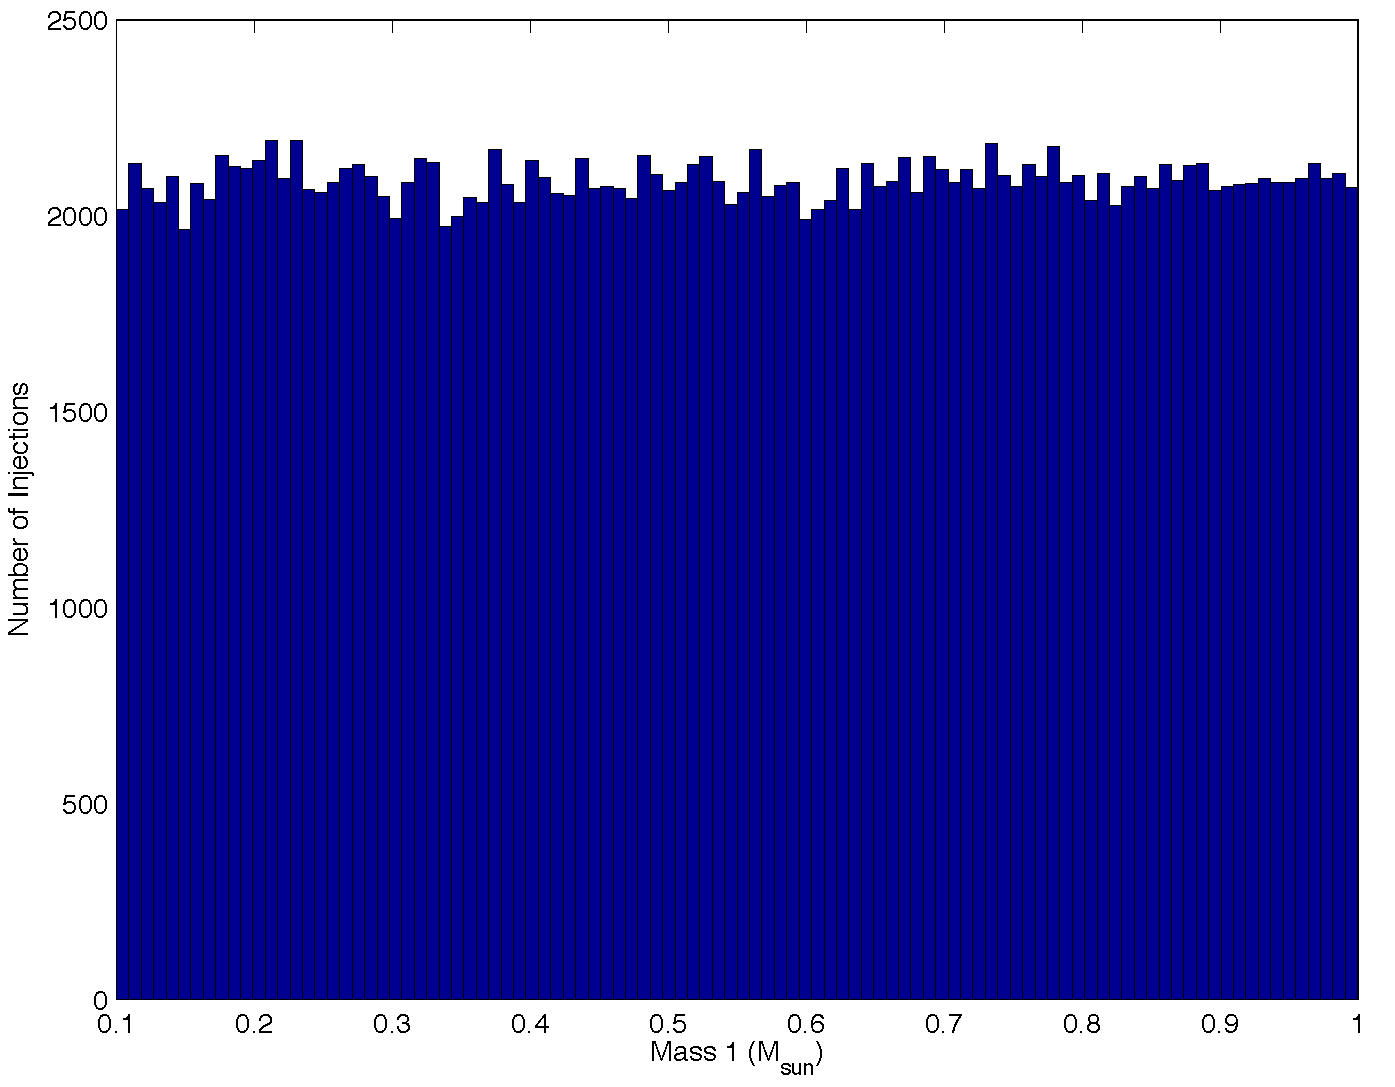
\includegraphics[width=\linewidth]{figures/macho/m1_hist}
\end{center}
\caption[Histogram of BBHMACHO Monte Carlo Mass Distribution]{
The BBHMACHO population Monte Carlo code is used to simulate a distribution of
$209048$ coalescing binaries and a histogram is made of the first component
mass, $m_1$ to confirm that it is uniformly distributed over the expected
range.  Similar tests are performed for the second mass parameter, $m_2$, the
galactocentric longitude, $\theta$, the inclination angle, $\iota$, the
polarization angle, $\psi$, and the coalescence phase, $\phi_c$.
}
\end{figure}

\begin{figure}[p]
\label{f:spherical_cartesian}
\begin{center}
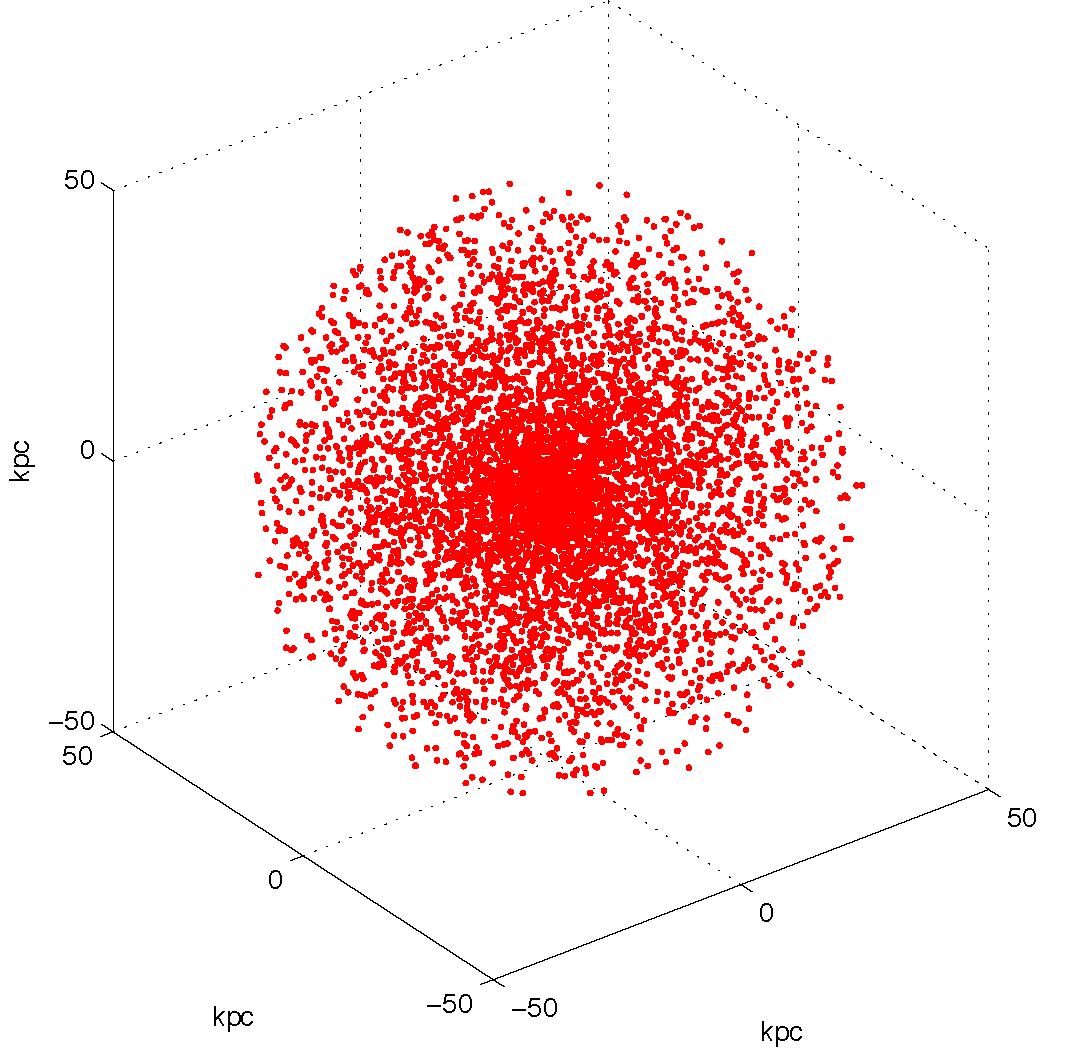
\includegraphics[width=\linewidth]{figures/macho/spherical_cartesian}
\end{center}
\caption[Spatial Distibution of Binary Black Hole MACHOs in Galactocentric
Coordinates]{%
The spatial distribution of $5000$ simulated BBHMACHO binaries in a spherical
$q=1$ Galactic halo of size $R_\mathrm{max} = 50\,\mathrm{kpc}$ with a core
radius $a = 8.5\,\mathrm{kpc}$ shown in galactocentric coordinates. Each point
in the figure corresponds to a simulated binary black hole MACHO injection.
}
\end{figure}

\begin{figure}[p]
\label{f:spherical_equatorial}
\begin{center}
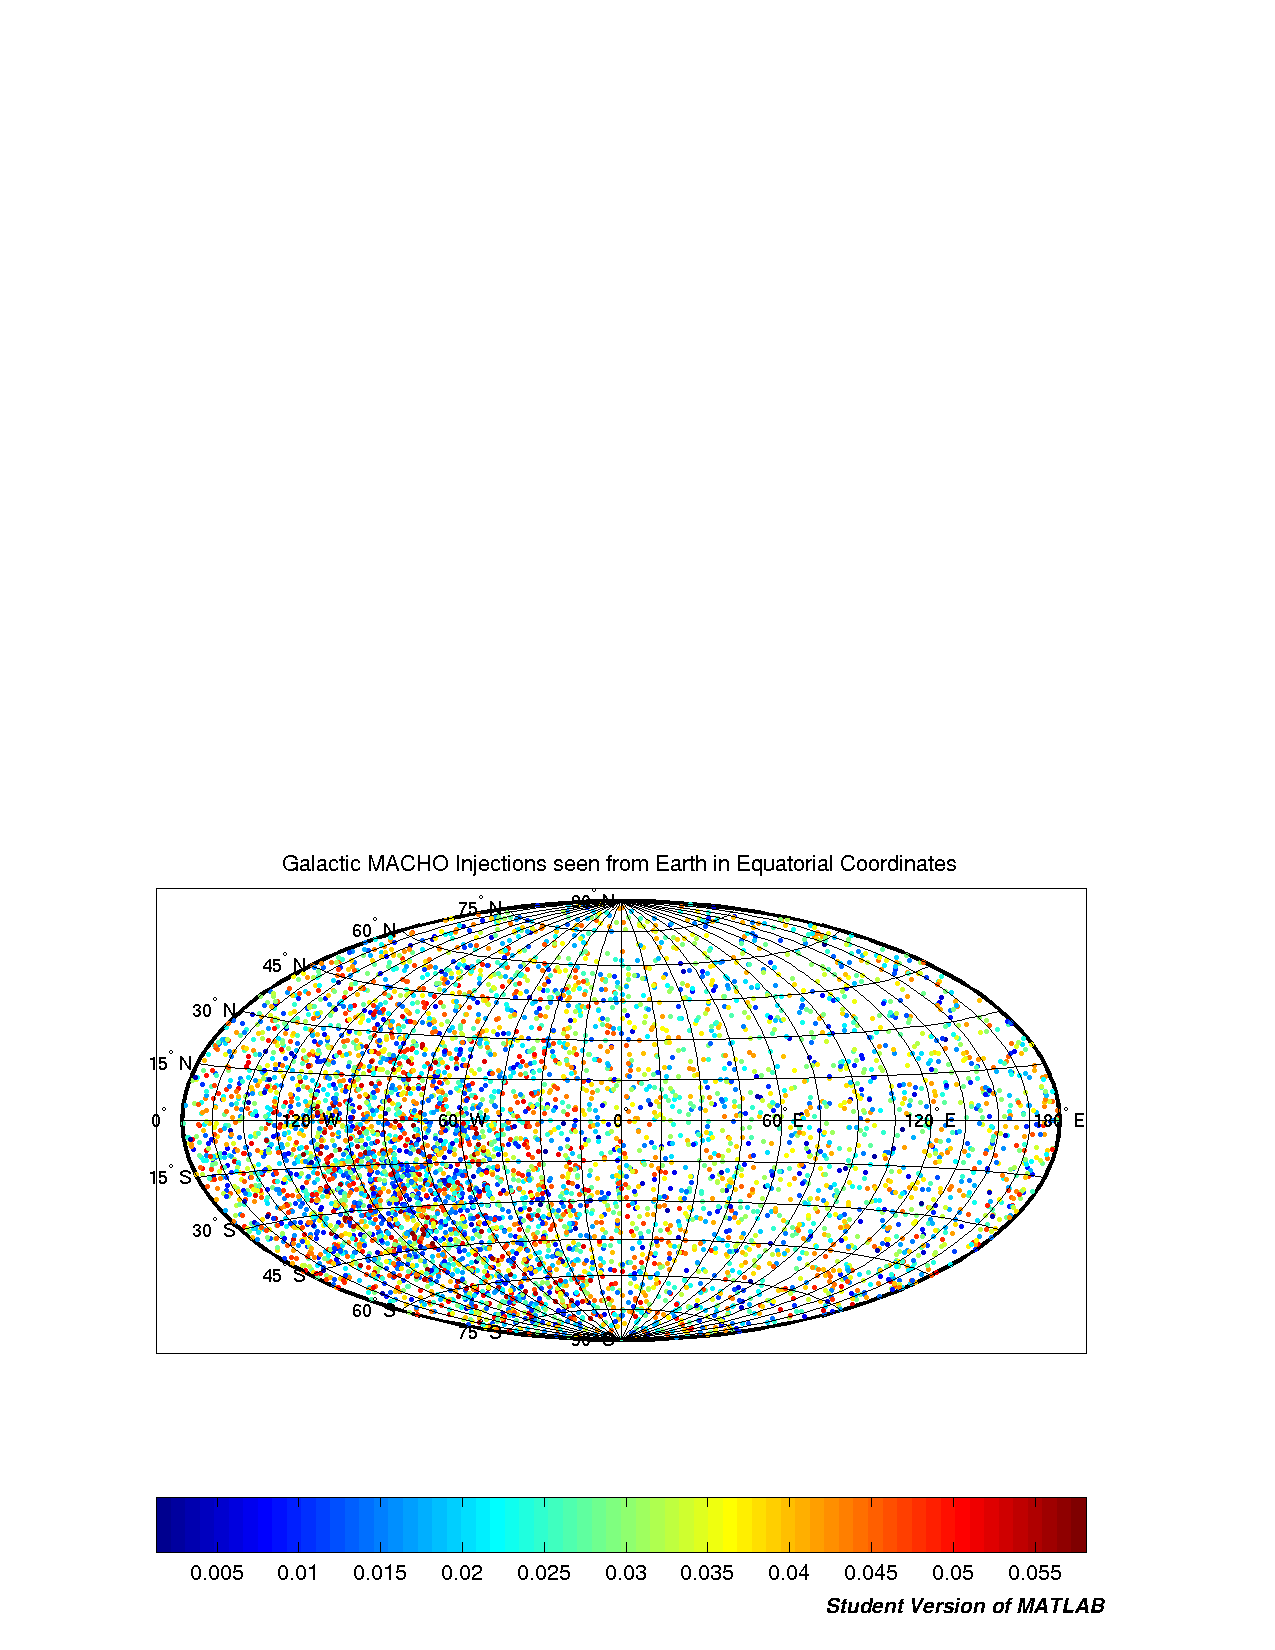
\includegraphics[width=\linewidth]{figures/macho/spherical_equatorial}
\end{center}
\caption[Spatial Distibution of Binary Black Hole MACHOS Seen From Earth]{
The spatial distribution of $5000$ simulated BBHMACHO binaries in a spherical,
$q=0$, Galactic halo of size $R_\mathrm{max} = 50\,\mathrm{kpc}$ with a core
radius $a = 8.5\,\mathrm{kpc}$ shown in equatorial coordinates. Each point
in the figure corresponds to a simulated binary black hole MACHO injection.
The color of the point shows the distance from the center of the earth to the
binary. Note the dense clump of binaries in the southern hemisphere, towards
the center of the Galaxy.
}
\end{figure}
